\documentclass{report}

\usepackage[12pt]{extsizes}

\usepackage[utf8]{inputenc}
\usepackage[T1]{fontenc}
\usepackage{natbib}
\usepackage{graphicx}
\usepackage[francais]{babel}
\usepackage{geometry}

\title{Solution de Streaming}
\author{Bastien Sauvan \and Paul Cocu \and François Le Nalio}
\date{Novembre 2015 à Juin 2016}

 \geometry{
 a4paper,
 total={210mm,297mm},
 left=25mm,
 right=25mm,
 top=25mm,
 bottom=25mm,
 }



 

\makeatletter
\def\thickhrulefill{\leavevmode \leaders \hrule height 1.2ex \hfill \kern \z@}
\def\@makechapterhead#1{
  \vspace*{10\p@}%
  {\parindent \z@ \centering \reset@font
        \thickhrulefill\quad 
        \scshape\bfseries\textit{\@chapapp{}  \thechapter}  
        \quad \thickhrulefill
        \par\nobreak
        \vspace*{10\p@}%
        \interlinepenalty\@M
        \hrule
        \vspace*{10\p@}%
        \Huge \bfseries #1 \par\nobreak
        \par
        \vspace*{10\p@}%
        \hrule
        \vskip 100\p@
  }}




% ENTETE ET PIED DE PAGE PERSONALISE

\usepackage{fancyhdr}
\pagestyle{fancy}

\renewcommand{\headrulewidth}{1pt}
\fancyhead[C]{\textit{\leftmark}} 
\fancyhead[L]{}
\fancyhead[R]{}

\renewcommand{\footrulewidth}{1pt}
\fancyfoot[C]{\textit{\thepage~sur \pageref{LastPage}}} 
\fancyfoot[L]{\textit{LP MERIT 2015/2016}}
\fancyfoot[R]{\textit{\LaTeX}}

\usepackage{lastpage}
\usepackage{fancyhdr} % for use of \pageref{LastPage}

\fancypagestyle{IHA-fancy-style}{%
  \fancyhf{}% Clear header and footer
  \fancyhead[LE,RO]{\slshape \rightmark}
  \fancyhead[LO,RE]{\slshape \leftmark}
  \fancyfoot[C]{\thepage\ sur \pageref{LastPage}}% Custom footer
  \renewcommand{\headrulewidth}{0.4pt}% Line at the header visible
  \renewcommand{\footrulewidth}{0.4pt}% Line at the footer visible
}

% Redefine the plain page style
\fancypagestyle{plain}{%
  \fancyhf{}%
  \fancyfoot[C]{\textit{\thepage\ sur \pageref{LastPage}}}%
  \fancyfoot[LE,RO]{\textit{\LaTeX}}
  \fancyfoot[LO,RE]{\textit{LP MERIT 2015/2016}}
  \renewcommand{\headrulewidth}{0pt}% Line at the header invisible
  \renewcommand{\footrulewidth}{0.4pt}% Line at the footer visible
}







\begin{document}

\maketitle





\begin{center}
\textbf{\Huge{Remerciements}}
\end{center}\\
\\
\\
\\
\hfill

Nous souhaitons avant toutes choses adresser nos plus sincères remerciements à l’ensemble des personnes qui nous ont permis d’effectuer ce projet tuteuré dans les meilleures conditions.
\\
\\
Nous remercions l’ensemble de l’équipe pédagogique de l’IUT de Créteil-Vitry pour leur disponibilité et leur écoute tout au long de cette année universitaire ainsi que leurs aide et leurs conseils techniques lors de la mise en place et la réalisation de notre projet.
\\
\\
Un remerciement particulier à Mr. DIAZ qui nous a suivi et supporté durant tout le projet et qui nous a fait part de son expertise technique au sujet de la diffusion de contenu multimédia.
\\
\\
Nous souhaitons également remercier Mr. SOUPRAMANIEN pour sa disponibilité, sa réactivité lors de la la mise en place du matériel dont nous avions eu besoin afin de réaliser notre projet.
\\
\\
Pour finir, on tient à remercier l'ensemble de la communauté présent sur le Github du module RTMP, et sur le site officiel du logiciel Open Broadcaster Software qui mettent régulièrement à jour leurs documentations qui est très clair et détaillé.  


\newpage

\begin{center}
\textbf{\Huge{Glossaire des figures}}
\end{center}\\

\hfill
\\



\textit{\underline{Figure 1.2} - Page 7 - Fonctionnement de l'Unicast contre le Multicast}
\\

\textit{\underline{Figure 1.3} - Page 12 - Documentation configuration de Base Serveur NGINX}
\\


\textit{\underline{Figure 2.3} - Page 12 - Documentation configuration du Pull Serveur NGINX}
\\


\textit{\underline{Figure 3.3} - Page 13 - Documentation configuration des Statistiques Serveur NGINX}
\\

\textit{\underline{Figure 3.3} - Page 13 - Documentation configuration des Statistiques Serveur NGINX}
\\

\textit{\underline{Figure 4.3} - Page 15 - Syntaxe JavaScript intégration lecteur Flash}
\\

\textit{\underline{Figure 5.3} - Page 17 - Architecture de test pour le LoadBalancing}
\\

\textit{\underline{Figure 6.3} - Page 17 - Configuration de test pour le LoadBalancing}
\\

\textit{\underline{Figure 1.4} - Page 18 - Schéma de l'architecture de notre solution}
\\

\textit{\underline{Figure 2.4} - Page 21 - Tableau des Canaux et Fréquences TNT nationale}
\\

\textit{\underline{Figure 3.4} - Page 26 - Extrait de la configuration de base RTMP Serveur NGINX1}
\\

\textit{\underline{Figure 4.4} - Page 27 - Extrait de la configuration finale RTMP Serveur NGINX1}
\\

\textit{\underline{Figure 5.4} - Page 28 - Extrait de la configuration HTTP Serveur NGINX}
\\

\textit{\underline{Figure 6.4} - Page 29 - Vérification de l'ajout du plugin sur OBS}
\\

\textit{\underline{Figure 7.4} - Page 30 - Ajout d'un flux réseau avec le plugin sur OBS}
\\

\textit{\underline{Figure 8.4} - Page 30 - Configuration de l'encodage sur OBS}
\\

\textit{\underline{Figure 9.4} - Page 31 - Configuration de diffusion sur OBS}
\\

\textit{\underline{Figure 10.4} - Page 32 - Code JavaScript pour intégrer le lecteur Flash}
\\

\textit{\underline{Figure 11.4} - Page 32 - Code JavaScript pour intégrer le lecteur Flash}
\\

\textit{\underline{Figure 12.4} - Page 34 - Extrait de la configuration finale du Serveur HAProxy}
\\

\textit{\underline{Figure 13.4} - Page 35 - Code JavaScript final pour intégrer le lecteur Flash}
\\

\textit{\underline{Figure 14.4} - Page 35 - Client VLC pour ouvrir notre flux en live}
\\







\tableofcontents

\chapter{Introduction}

Notre projet tuteuré s’inscrit dans le cadre de notre licence professionnelle “Métiers des Réseaux Informatiques et Télécommunications” à l’IUT de Créteil-Vitry.
\\
\\
Notre groupe de projet est composé de Bastien Sauvan, François Le Nalio et Paul Cocu. Le but de notre projet étant de mettre en oeuvre nos connaissances dans le domaine de la diffusion de contenue Multimédia.
\\
\\
En effet, le but de notre projet est de mettre en place une solution de Streaming.
\\
\\
Ce projet est né de l'intérêt que porte l’un des membres du groupe pour les technologies de Streaming. De plus les technologies de Streaming sont en pleine expansion avec l'émergence de plate-forme telle que YouTube Gaming, Twitch, Daylimotion etc…
\\
\\
La nature de ce projet est en parfait accord avec l'option que nous avons choisi pour notre année de Licence Professionnelle : Administration des Réseaux Multimédia.
\\
\\
Une fois notre projet définie il fallait également définir une possible application à la mise en place d'un telle solution.
\\
\\
Après réflexions nous avions envisager plusieurs scénarios possible : 
\\

   \begin{itemize}
       \item Assurer la retransmission en live d'une conférence
       \item Assurer la retransmission en live d'un cours universitaire
       \item Assurer la retransmission en live d'un évènement à but non lucratif
   \end{itemize} 


\hfill{\\}
Mais après un premier entretien avec Mr. DIAZ, il nous a proposer de mettre en place dans l'université une retransmission de l'Euro 2016 commençant début Juin.
\\
\\
Nous avons alors aussitôt relevé le défi, pensant que c'était une bon choix d'application pour la mise en place d'une telle solution.



\chapter{Recherche de solutions}
   
    \section{Topologie de diffusion}
    
    Il est essentiel de s'intéresser dans un premier temps  aux différentes topologie de diffusion existante dans le monde des réseaux. Quel type de routage sera le meilleur choix pour notre type d’application réseau.
    \\
    \\
    En effet, en réseau  le routage est le mécanisme par lequel des chemins sont sélectionnés dans un réseau pour acheminer les données d'un expéditeur jusqu'à un ou plusieurs destinataires. 
    \\
    \\
    Il faudra prendre en compte certaines problématiques comme la saturation de la bande passante, où encore la qualité de transmission des flux Streaming.


        \subsection{Broadcast}
     
        
    \underline{Description}
    \\
    
    \\
    La notion de broadcast est employée par les techniciens en informatique et réseaux ; il s'agit à proprement parler, de transmission ou de liaison. 
    Le principe de base est le même que la télédiffusion, étant donné que l'on diffuse des paquets de données à de nombreux clients éventuellement sans discrimination.    \\
   
    \\
    \underline{Avantages}
    \\
   \begin{itemize}
       \item Aucun avantages de cette méthode de diffusion
   \end{itemize} 
    \\
    \hfill
    
    \underline{Inconvénients}
    \\
   \begin{itemize}
       \item Saturation du réseaux
       \item Pas du tout adapté au Streaming
       \item L'étendue de diffusion sera restreinte au domaine de diffusion
   \end{itemize} 
    \\
    \\
    
    \hfill{\\}
    
        \subsection{Multicast}
        
  \underline{Description}
    \\
    
    \\
   Le multicast est une forme de diffusion d'un émetteur vers un groupe de récepteurs. Les récepteurs intéressés par les messages adressés à ce groupe doivent s'abonner au flux. Ces abonnements permettent aux switchs et routeurs intermédiaires d'établir une route depuis le ou les émetteurs de ce groupe vers les récepteurs de ce groupe.
    \\
    \\
    Le multicast est donc utiliser dans des applications interactives de groupe, comme la visioconférence, le partage de tableau, la diffusion de contenue multimédia...
    \\
   
    \\
    \underline{Avantages}\\
   
   Ce système est plus efficace que l'unicast pour diffuser des contenus simultanément vers une large audience. En multicast, chaque paquet n'est émis qu'une seule fois et sera routé vers toutes les machines du groupe de diffusion sans que le contenu ne soit dupliqué sur une quelconque ligne physique ; c'est donc le réseau qui se charge de reproduire les données.
    \\
    \\
    Le multicast permet alors de préserver la bande passante du réseau. 
    \\
  
    \\    
    \underline{Inconvénients}\\
    
    Mais le multicast ne permet cependant en aucune façon le contrôle de la participation au groupe par la source : la source ne peut déterminer ni qui participe, ni qui peut participer ou non au groupe.
    \\
    \\
    Et surtout le gros inconvénient du Multicast est que les routeurs doivent être configurés de telle manière à gérer le multicast. Survient alors le probleme sur internet de faire du Multicast, car en effet, nous n’avons pas la main sur tous les routeurs que nous traversons.
    \\
    \\
    C’est donc pour ça que le multicast sur internet est très rare et très compliqué, les grosses plates-formes de Streaming, n’utilisent pas le Multicast.

    \\
   
    \\
        \subsection{Unicast}
   
     \underline{Description}
    \\
    
    \\
     Le terme unicast définit une connexion réseau point à point, c'est-à-dire d'un hôte vers un (seul) autre hôte.
    \\
    \\
    On entend par unicast le fait de communiquer entre deux ordinateurs identifiés chacun par une adresse réseau unique. Les paquets de données sont routés sur le réseau suivant l'adresse du destinataire encapsulée dans la trame transmise. Normalement, seul le destinataire intercepte et décode le paquet qui lui est adressé.
    \\
       \hfill{\\\\\\}

    \\
    \underline{Avantages}\\
    
    L’avantage de l’unicast se retrouve dans la gestion et le contrôle que l’on a entre la source et les récepteurs. En effet nous sommes libres de contrôler qui à accès à la source ou non.
    \\
  
    \\    
    \underline{Inconvénients}\\
    
    En streaming unicast, on enverrait l'information autant de fois qu'il y a de connexions, d'où un gaspillage de temps, de ressources du serveur et surtout de bande passante du réseau.	
    
    \\
    \begin{center}
    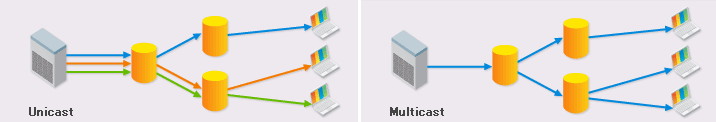
\includegraphics[width=16cm]{img/uni.png}
    \textit{\small{Cette figure représente bien l'avantage du Multicast contre l'Unicast}}
    \end{center}

    
    
        \subsection{Notre choix}
    
   Comme nous avons pu le voir précédemment, le Broadcast n’est pas du tout adapté pour faire du streaming, et en théorie le meilleur choix se porterait vers le Multicast. Mais il reste très compliqué à mettre en oeuvre pour un service sur internet. Or notre projet à pour objet de reproduire un service qui pourrait être mis en production sur une application réelle, donc potentiellement sur Internet. C’est pour cette raison que nous avons choisi d’utiliser le type de diffusion : Unicast.	

    
    \section{Solutions Streaming trouvées}    
        
        \subsection{VLC}
     
        
    \underline{Description}
    \\
    
    \\
    VLC media player (VLC) est un lecteur multimédia libre. Ce logiciel est multi-plateforme puisqu’il fonctionne sous plus de 20 plates-formes. L’ayant vaguement étudié en première année nous savions qu’il était possible de l’utiliser pour faire du Streaming. De là, nous avons approfondi nos recherches pour définir réellement comment nous pourrions utiliser VLC.
    \\
    \\
    Ce qui fait la puissance de VLC, et ce qui va nous intéresser particulièrement pour notre application, c’est que VLC peut se comporter aussi bien en tant que Client mais aussi en tant que Serveur. Un des autres grands atouts de VLC est que le lecteur est capable de lire un grand nombre de flux réseaux mais aussi qu’il intègre les codecs nécessaires à la lecture de la plupart des formats audio et vidéo.
    \\
   
    \\
    \underline{Avantages}\\
    
    Dans nos recherches, nous avons alors compris qu’il était possible avec VLC de : Lire, Diffuser ou Convertir des Fichiers, Disques, Flux Réseaux, mais aussi des périphériques de captures (vidéo et audio).
    \\
    \\
    \\
    Il est possible de diffuser avec une ou plusieurs méthodes : Fichier, HTTP, MS-WMSP, RTSP, RTP, UDP,Icecast.
    \\

    Il est possible de transcoder avec les paramètres suivants :
    \\

   \begin{itemize}
    \item Plusieurs méthodes d’encapsulation :MPEG, Ogg, MP4, WAV, MKV, AVI, FLV
    \item Plusieurs codecs vidéo : MPEG, DIVX, Théora, H264 en choisissant le débit souhaité.
    \item Plusieurs codecs audio : MPEG, MP3, FLAC, WAV, Vorbis en ayant la possibilité de choisir le débit et la fréquence d’échantillonage.
    \end{itemize} 
    \\
    \hfill{\\}

    \underline{Inconvénients}\\
    
    Mais après avoir vu les nombreuses possibilités que nous offre VLC, nous nous sommes vite rendus compte qu’il n’allait pas pouvoir faire tout ce que l’on souhaitait pour mettre en place un service de Streaming
    \\
    \\
    En effet, VLC peut faire énormément de choses avec un flux vidéo ou audio, mais il ne sait traiter à la fois qu’un seul et unique flux. Chaque instance de VLC ne peut gérer qu’un flux. 
    \\
    \\
    Nous avons donc continué nos recherches pour trouver une solution plus adaptée au Streaming de masse.


        \subsection{Icecast}
    
        
    \underline{Description}
    \\
    
    \\
    Icecast est un logiciel libre (sous licence GPL) de type serveur de diffusion de flux (streaming), audio et vidéo. Il permet donc à partir d'un ordinateur (sous Windows, GNU/Linux, Mac OS X ou autre) de diffuser de la musique et des vidéos à des logiciels « clients » (lecteurs audio ou multimédias), au travers d'Internet ou d'un intranet (réseau local). Il génère également une interface web dynamique qui permet d'administrer le serveur.
    \\
   
    \\
    \underline{Avantages}\\
    
    Facile à mettre en oeuvre / Open Source et Gratuit / Site communautaire Forum etc
     \\
     Le serveur Icecast est capable de produire un flux dans les formats suivants à travers les protocoles HTTP et HTTPS : 
    \\
    

  
    \underline{Inconvénients}\\
    
    Le serveur Icecast est capable de produire un flux dans les formats suivants à travers les protocoles HTTP et HTTPS : 
    \\

    
    \begin{itemize}
    \item Audio : Ogg (Vorbis, Opus, Speex, CELT), AAC, MP3, Skype SILK.
    \item Vidéo : Ogg Theora, WebM, Nullsoft Streaming Video (en).
    \end{itemize} 


    \hfill
    \\
    Or ces codecs ci dessous sont très limités pour faire de la vidéo, et les protocoles HTTP et HTTPS pas adaptés pour faire du Streaming.
    
        \subsection{Adobe Flash Media Server}
    
        
    \underline{Description}
    \\
    
    \\
    Flash Media Server (FMS) est un produit commercial serveur d'Adobe Systems Inc. (qui a racheté Macromedia). Ce serveur fonctionne avec le lecteur Flash pour permettre des animations interactives, multi-utilisateurs : Rich Internet Applications). 
    \\
    \\
    \begin{itemize}
    \item Diffusion de vidéo préenregistrée (Video on Demand, streaming) ou non, webcam
    \item Communication par vidéo (son et images) en temps réel entre plusieurs clients : chat room ou jeu multijoueur.
    \end{itemize}
    \\
    \\
    Flash Media Server est un hub, Les applications clientes se connectent sur le hub en utilisant le protocole Real Time Messaging Protocol (RTMP). 
    \\
    \\
    Les clients peuvent créer un canal de diffusion vidéo ou déposer leurs vidéos sur le serveur au format Flash Video (FLV).
    \\
   
    \\
    \underline{Avantages}

    \\
    \\
    \begin{itemize}
    \item Simple à prendre en main pour faire sa diffusion
    \item Service de qualité
    \item QOS
    \end{itemize}
  
    \\    
    \underline{Inconvénients}
    
    \\
    \\
    \begin{itemize}
    \item Propriétaire
    \item Solution coûteuse
    \item Pas de prise en main des serveurs, on paye pour un service
    \end{itemize}
    
        \subsection{Nginx}
    
        
    \underline{Description}
    \\
    
    \\
    Tout au long de nos études informatiques et réseaux nous avons déjà étudié, configuré et mis en place un serveur HTTP pour une application Web.
    \\
    \\
    Nous avions alors vu qu’il était possible d’ajouter certains modules afin d’utiliser certains protocoles.
    \\
    \\
    Après nos recherches, on a pu constater qu’un serveur HTTP fait concurrence actuellement au célèbre “Apache2”, celui-ci se nomme “NGINX”. Ce dernier est reconnu pour sa simplicité et ses performances, notamment sur le taux de transfert en fonction du nombre de clients connectés simultanément.
    \\
    \\
        \hfill{\\}


    En continuant nos recherches, nous avons pu comprendre que relativement aux performances du Serveur NGINX, un module a été développé pour implémenter l’utilisation du protocole RTMP, le protocole de Streaming que l’on a vu précédemment sur la solution Adobe.
    \\
    \\
    Le protocole RTMP est utilisé par toutes les plus grandes plates-formes de Streaming actuelles telles que : Twitch, Daylimotion, YouTube, etc.
    \\
    \\
    Ce module RTMP permettrait alors la gestion de flux de Streaming
    \\
   
    \\
    \underline{Avantages}\\
    
    \begin{itemize}
    \item Open Source et Free
    \item Performance
    \item Module Open Source pour RTMP
    \item Compatible sur Debian
    \item Documentation complète
    \end{itemize}

    \hfill{}

    \underline{Inconvénients}\\
    
    Nécessite des connaissances en Linux


    

        \subsection{Notre choix}\\
        
    Au vu des différentes solutions trouvées, notre choix s'est porté vers la mise en place de NGINX.
    \\
    \\
    Cette solution nous semble la plus adaptée pour l'objectif de notre projet.
    \\
    \\
    En effet, cette solution s'apparente au mieux à la mise en place d'un service de Streaming industriel comme on peut retrouver sur Internet.
    \\
    \\
    Derrière notre plate-forme de Streaming maison, on pourra alors retrouver des Serveurs NGINX exploitant le protocole de Streaming RTMP.
    
    
    \\
    \\


\chapter{Étude pratique}
    \section{Streamers Ikusi}
    Pour rappel, l’objectif de notre projet est de diffuser la retransmission des matchs de l’Euro 2016, il sera donc nécessaire de récupérer les flux TNT des chaînes responsable de la retransmission des matchs.
    \\
    \\
    Pour cela, nous avons vu lors d’un TP en module de "Vidéotransmission et télésurveillance" que nous pouvions utiliser les Streamers de la marque IKUSI présents en salle 201.
    \\
    \\
    IKUSI est une société espagnol pionnière dans le développement de solutions de traitement numérique de signaux de vidéo et télévision destinées aux opérateurs, aux grands installateurs, aux intégrateurs et au secteur professionnel de la distribution d'équipements électroniques.
    \\
    \\
    Notre salle 201 de TP est équipée de 6 Streamers prêts à l'emploi.
    \\
    \\
    

    Ces Streamers sont reliés a une antenne TNT pour recevoir les chaînes TNT.
    \\
    \\
        
    \begin{itemize}
    
    \item Ils sont capables de gérer une bande de fréquence
    \item Ils diffusent sur un réseau IP uniquement en Multicast
    \item Ils gèrent les protocoles RTP et UDP
    \item Ils peuvent diffuser un flux unique
    \item Ils peuvent diffuser un flux multiplexé (TS)
    \end{itemize}
    \\
    \hfill
    \\
    \begin{center}
    \textbf{\textit{On verra lors du déploiement de notre solution quelles fréquences et quel protocole nous allons utiliser.}}
    \end{center}
    
    \section{NGINX} 
    Comme on a pu le voir précédemment, parmi les solutions trouvées, nous avons choisi d’utiliser des serveurs NGINX qui vont tourner sous Linux.
    \\
    \\
    NGINX est compatible avec la distribution de Linux utilisé ici : Debian. On verra que l'installation des serveurs se fera sur la version Wheezy de Debian.
    \\
    \\
    
    On retrouve au coeur d’un service de Streaming des serveurs dédiés à la diffusion des flux vidéos et audio. Il était donc nécessaire d’appréhender au mieux le coeur de notre projet en se documentant et en testant les serveurs qui allaient être responsables de la gestion des flux.
    \\
    \\
    Cette fonction va être assuré par les serveurs NGINX couplé à un module pour implémenter sur le serveur l’utilisation du protocole de Streaming : RTMP
    \\
    \hfill
    Il était donc nécessaire de se renseigner un maximum sur la technologie.
    \\
    \\
    RTMP est un protocole dédié pour la diffusion de données en streaming entre un serveur et un client. RTMP est basé sur TCP et exploite le port 1935. On notera également que le principale client pour lire un flux RTMP est un lecteur Flash.
    \\
    \\
    Pour comprendre le fonctionnement technique du module nous nous sommes rendu sur le dépôt officiel du module RTMP sur Github (voir Webographie). Sur ce même dépôt Github on retrouve une documentation, un wiki complèt sur toutes les fonctionnalités du module et des exmples de syntaxe pour mettre en pratique.
    \\
    \\
    Parmi celles-ci, certaines fonctionnalités paraissent essentielles pour notre service de Streaming :
    \\
    \\
    
    \begin{center}
    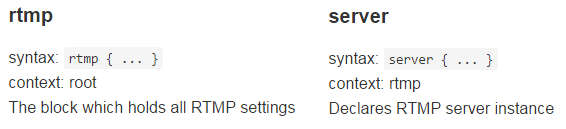
\includegraphics[width=16cm]{img/nginx3.PNG}
    \textit{\small{On retrouve dans la documentation comment nous allons écrire notre configuration}}
    \end{center}
    \\
    \\
    
    \begin{center}
    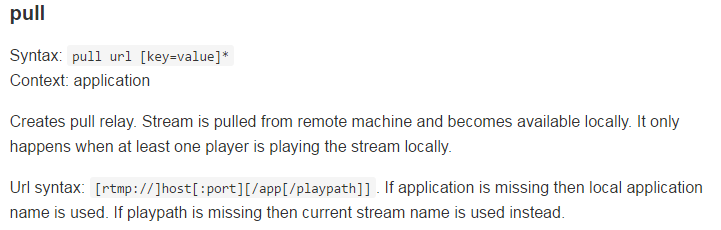
\includegraphics[width=16cm]{img/nginx1.PNG}
    \textit{\small{On retrouve dans la documentation une fonctionnalitée de pull un flux RTMP}}
    \end{center}

    \\
    \hfill{\\\\}
    
    \begin{center}
    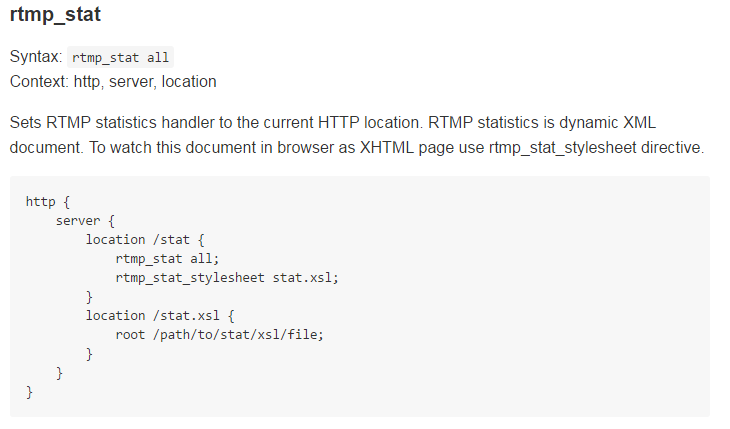
\includegraphics[width=16cm]{img/nginx2.PNG}
    \textit{\small{On retrouve dans la documentation une fonctionnalitée de statistiques sur le serveur}}
    \end{center}

    \\
    \hfill{\\\\}

    \begin{center}
    \textbf{\textit{ On verra lors du déploiement de notre solution la configuration précise de nos serveur et les fonctionnalités que nous allons mettre en place sur nos serveurs.}}
    \end{center}

    \hfill{\\\\}

    \section{Open Broadcaster Software (OBS)} 
    
    \underline{Etudes sur OBS:}\\
    
    Sur le site officiel, voir webographie, nous avons alors chercher un maximum d’information sur le logiciel.
    \\
    \\
    OBS est un logiciel gratuit et Open source de diffusion et d'enregistrement vidéo. Il s'agit aussi d'un logiciel communautaire qui est encore en évolution. Amateurs de Jeux vidéos, nous connaissions déjà ce logiciel qui est utilisé par de nombreux Streamers indépendants que nous suivons régulièrement sur les plates-formes de Streaming.\\

    \\
    \underline{Remarques:}\\
    
    OBS est simplement un logiciel de mixage vidéo et audio. En aucun cas le logiciel peut faire serveur de Streaming.\\

    \\
    \underline{Plugin Source Vidéo:}\\
    
    
    Dans notre découverte des différents plugins existants, nous avons vu qu’il existait un plugin nommé : Video source plugin
    \\
    \\
    On retrouvera dans la Webographie le lien officiel du plugin.
    \\
    \\
    Et qu’avec ce plugin, tout comme avec VLC par exemple, il était possible d’ouvrir des flux Réseaux.
    \\
    \\
    Après quelques tests on a pu constater que ce plugin gère les protocoles suivants :
    \\


    \begin{itemize}
    \item UDP
    \item RTP
    \item RTMP
    \end{itemize}

    \hfill
    \\
    Nous avons alors compris que ça allait nous être très utile sur notre régie pour ouvrir les flux de nos Streamers.\\
    
    
    \underline{Test diffusion Serveur NGINX:}\\
    
    D’après nos recherches, ce logiciel est compatible avec le protocole RTMP, car en effet on peut utiliser ce logiciel pour Stream vers les grosses plates-formes de Streaming comme Twitch par exemple qui utilise le protocole RTMP.
    \\
    \\
    Nous avons alors testé ce logiciel pour diffuser vers notre serveur de Streaming NGINX.
    \\
    \\
    \begin{center}
    \textbf{\textit{On verra lors du déploiement de notre solution la configuration du logiciel que nous avons réalisée, et sur quels paramètres précisément nous allons jouer pour optimiser notre flux de Streaming.}}
    \end{center}
    

    \section{Intégration lecteur Flash}  
    \\
    \\
    Pour nos futurs clients, il est nécéssaire qu’il puisse accéder au live via une interface graphique. Pour cela, il faut donc que l’on teste si on peut intégrer notre live sur une page Web.
    \\
    \\
    \underline{Mise en place d’un site de test en local :}\\
    
    Pour tester l’intégration d’un lecteur, nous avons mis en place un site Web local qui nous servira de test. Nous avons alors monté un Apache2 classique sur une machine en salle 201.
    \\
    \\
    \underline{Intégration d’un lecteur:}\\
    
    Le protocole que l’on utilise pour notre flux de Streaming (RTMP) n’est toujours pas compatible avec HTML5, par contre il est compatible avec un client Flash.
    \\
    \\
    En effet, certains lecteurs Flash sont capables d’ouvrir des flux RTMP en temps réel.
    \\
    \\
    Nous avons donc testé l’intégration d’un des lecteurs flash les plus connus (JWPlayer) que l’on avait préalablement vu lors d’une séance de TP en vidéotransmission.
    \\
    \hfill{\\\\}
    
    \underline{Test de lecture d’un flux:}\\
     
    Une fois le lecteur intégré sur la page Web de test, nous avons donc essayé de lire le flux de Streaming que l’on avait préalablement mis en place pour l'occasion.
    \\
    \\
    A l’aide de la documentation officiel le site constructeur nous avons pu vérifier le bon fonctionnement de la lecture de notre flux.
    \\
    \begin{center}
    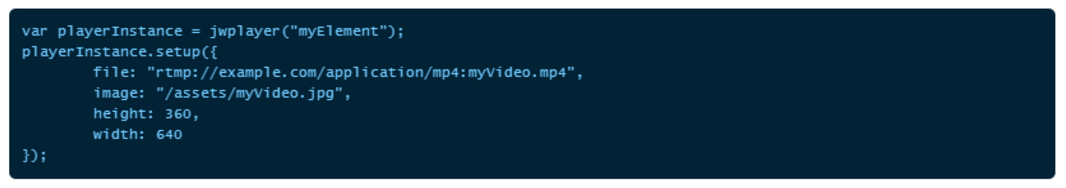
\includegraphics[width=16cm]{img/jwplayer1.PNG}
    \textit{\small{On retrouve ici la syntaxe JavaScript pour intégrer le lecteur et lire notre flux RTMP}}
    \end{center}

    
    \hfill{\\}
    
    \begin{center}
    \textbf{\textit{On verra lors du déploiement de notre solution quelle sera le code final de notre lecteur Flash}}
    \end{center}
    \\
    
    \hfill{\\}
    
     \underline{Test de différentes options:}\\
     
    Également avec la documentation constructeur sur leur lecteur on a pu trouver la possibilité d’utiliser des options telles que :

    \begin{center}
    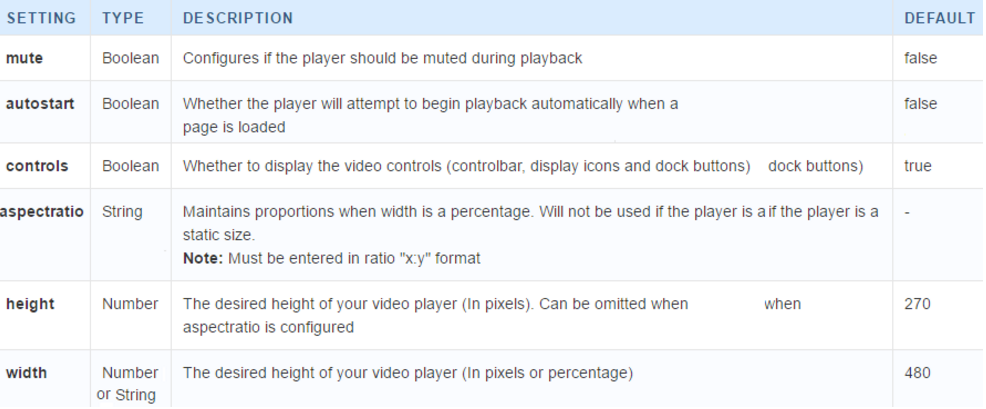
\includegraphics[width=16.5cm]{img/jwplayer.PNG}
        \end{center}
    
    \\
    
    \begin{center}
    \textbf{\textit{ On verra lors du déploiement de notre solution quelles options nous allons utiliser pour paramétrer notre lecteur.}}
    \end{center}
    \\
    \hfill

    
    \section{LoadBalancing}  
    
    \underline{Pourquoi étudier le LoadBalancing ?}\\

    La gestion de flux de Streaming nécessite de la puissance de calcul, ainsi que de la bande passante. Il était alors important de se questionner sur la répartition de la charge lors de la mise en place d’une solution de Streaming.\\
    
    
    \underline{Quel serveur de LoadBalancing ?}\\
    
    Pour rester dans le milieu de l’OpenSource nous souhaitions utiliser HAProxy connu pour sa stabilité, et ses bonnes performances. 
    \\
    \\
    HAProxy est un serveur permettant de faire du LoadBalancing, de la haute disponibilité mais aussi du reverse proxy TCP et HTTP.\\
    
    \underline{Pourquoi étudier le LoadBalancing ?}\\
    
    
    Pour un peu mieux comprendre l’utilisation de HAProxy et prendre en main le serveur, nous avons fait un premier test pour faire du Load Balancing sur deux Serveurs Web.
    \\
    \\
    
    \hfill
    
    Ainsi, en joignant l’adresse IP du LoadBalancer, nous tomberons une fois sur le site WEB1 une fois sur le site WEB2, en fonction de comment le LoadBalancer va répartir la charge.
    \\
    \\
    Pour se faire, nous avons installé deux serveurs Web de test, et un serveur HAProxy, avec une configuration basique. La répartition de la charge se faisait bien sur les deux serveurs.
    \\
    \\

    \begin{center}
    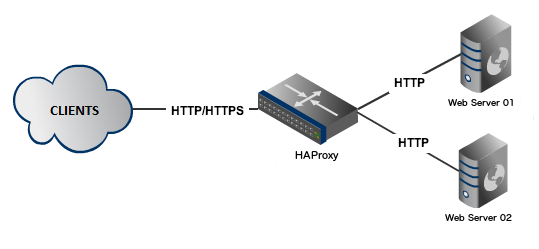
\includegraphics[width=14cm]{img/lb2.png}
    \\
    \textit{\small{On retrouve ici l'architecture mise en oeuvre pour tester le LoadBalancing}}
    \end{center}
    
    \hfill
    
    \begin{center}
    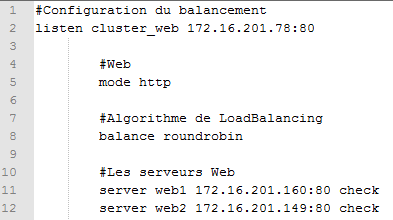
\includegraphics[width=13cm]{img/lb.PNG}
    \\
    \textit{\small{On retrouve la configuration de test sur notre Serveur de LoadBalancing}}
    \end{center}
    
    
    \hfill
    
    \begin{center}
    \textit{On verra lors du déploiement de notre solution la manière dont nous allons adapter la configuration du HAProxy pour nos flux de Streaming.}
    \end{center}
    
    
    
    
    
    
\chapter{Mise en oeuvre de la solution}
    \section{Architecture choisie}  
    
    \underline{Architecture choisie}\\
    
    \begin{center}
    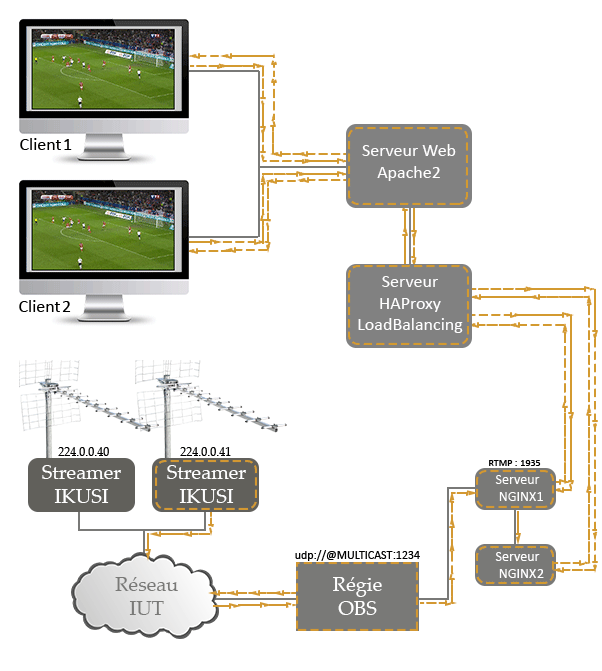
\includegraphics[width=13.5cm]{img/schema.png}
    
    \textit{\small{Figure 1.4}}
    \end{center}    
    \underline{Description de l’architecture ?}\\
    
    \begin{enumerate}
    \item  Nous devons dans un premier temps utiliser les Streamers de la Salle 201 pour récupérer les flux TNT et les diffuser sur le réseau de l’IUT (Protocole RTP).
    \item Il faudra ensuite mettre une machine pour faire une régie. Cette machine va utiliser le logiciel OBS qui va nous permettre de récupérer les flux TNT. On verra que cette machine aura deux cartes réseaux, une qui sera sur un réseau local pour récuperer les flux Multicast des Streamers, et une autre carte réseau sur le réseau de l'IUT pour pouvoir diffuser vers nos Serveurs NGINX (Protocole RTMP).
    \item Une fois le flux récupéré par le premier Serveur NGINX, le flux sera dupliqué vers le deuxième serveur NGINX. Une fois le flux disponible sur les deux serveurs, les serveurs sont prêts à diffuser le flux aux clients (Protocole RTMP).
    \item Les clients pourront se connecter sur notre plate-forme Web, sur notre serveur Apache2 (Protocole HTTP).
    \item Une fois sur la plate-forme Web les clients pourront lire le flux de Streaming via un lecteur Flash (Protocole RTMP).
    \item Lorsqu’un client demande le flux via le lecteur Flash il passe par le HAProxy qui LoadBalance une fois sur deux sur chaque Serveur NGINX.
    \end{enumerate}
    \\
    \hfill
    
    \underline{Pourquoi deux serveurs NGINX ?}\\
     
     
	Le trafic des flux sur le serveur consomme des ressources sur la machine. En effet, au plus de clients demandent le flux, au plus le serveur va devoir envoyer d’informations et donc va consommer des ressources CPU et de la bande passante. 
	\\
	\\
	Nous devons donc prévoir que notre solution de Streaming soutienne une certaine charge de clients, pour assurer une bonne qualité et une bonne répartition de la charge, nous avons donc prévu deux serveurs NGINX avec un LoadBalancer qui équilibrera la charge sur les deux serveurs.\\
	\\
	
	\underline{Matériel demandé ?}\\
	
	Nous avons présenté cette architecture à Mr. SOUPRAMANIEN en demandant pour notre projet :
	\\
	\\
	\begin{itemize}
    \item Une machine physique en salle 201 sur Windows 7 avec une carte vidéo dédié qui sera chargée de récupérer le flux du Streamer IKUSI et de le renvoyer sur nos serveurs.

    \item Deux serveurs au cœur du réseau sur Debian 7 avec des liens Gigabit si possible car ce sont eux qui seront responsables de l'envoi des flux en Unicast à tous les clients.

    \item Un serveur également au cœur du réseau sur Debian 7 qui hébergera notre plate-forme Web, ainsi que notre Load Balancer pour équilibrer la charge sur nos deux serveurs.
    \end{itemize}
    \\
    \\
    
    \hfill
    
    Mr. SOUPRAMANIEN nous a donc mis à disposition :
    \\
    \\
    \begin{itemize}
    \item 1 PC physique en salle 201 sur Windows 7
    \\
    \\
    \item 3 VM au coeur du réseau sur Debian Wheezy  (accès SSH)
    \end{itemize}
    \\
    \\
    \section{Configuration des Streamers}  
    \\
    \\
    Dans cette partie nous allons voir comment nous avons configuré les Streamers de l’IUT en salle 201 pour pouvoir récupérer les flux TNT et les diffuser sur le réseau de l’IUT.
    \\
    \\
    
	\underline{Choix du nombre de Streamer :}\\
	
	
    Pour commencer nous avons regardé le programme des chaînes de télévision en charge de diffuser les matchs et du contenu en rapport avec l’Euro 2016.
    \\
    \\
    Nous avons donc défini qu’il était judicieux au vu des éléments collectés de diffuser les trois chaînes suivante :
    \\
    \\
    \begin{itemize}
    \item TF1
    \item M6
    \item L’équipe 21
    \end{itemize}
    
    \hfill
    
    \\
    Or ces trois chaînes sont disponibles sur trois fréquences différentes, en effet d’après :
    \\
    \begin{center}
    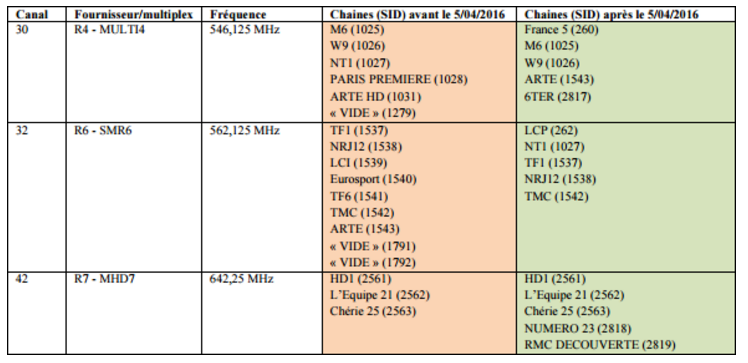
\includegraphics[width=16cm]{img/freq.PNG}
    
    \textit{\small{Figure 2.4}}
    \end{center}
    
    
    \hfill

    Chaîne  \rightarrow Fournisseur/Multiplex \rightarrow Fréquence
    \\
    
    TF1  \rightarrow R6 - SMR6 \rightarrow  562,125 MHz
    \\
    
    M6  \rightarrow R4 - MULTI4 \rightarrow 546,125 MHz
    \\
    
    L'équipe 21\rightarrow R7 - MHD7 \rightarrow  642,25 MHz
    \\
    \\
    
   
    Et comme nous l’avons vu au préalable dans les tests que l’on a pu faire avec les Streamers, il est possible de calibrer le Streamer sur une seule borne de fréquence. 
    \\
    \\
    Nous allons donc configurer et utiliser 3 Streamers différents pour chaque bande de fréquence.
    \\
    \\
    
    \underline{Interface d’administration Web des Streamer :}\\
    
    Comme nous l’avons vu pendant les tests, l’administration des Streamers IKUSI se fait via une interface Web. Par défaut l’adresse du Streamer est : 192.168.1.4 
    \\
    \\
    Or étant donné que nous avons 3 Streamers à administrer nous avons donc changé l’adresse des Streamers suivant le plan d’adressage suivant :
    \\
    \\
    
    -Streamer Tab4  \rightarrow  562,125 MHz \rightarrow   192.168.1.4
    \\
    
    -Streamer Tab5  \rightarrow  546,125 MHz \rightarrow   192.168.1.5
    \\
    
    -Streamer Tab6  \rightarrow  642,25 MHz \rightarrow   192.168.1.6
    \\
    \\
    
    \underline{Choix du protocole de diffusion :}\\
    
    Nous avons vu que le Streamer est capable d'en-capsuler le flux soit en UDP soit en RTP. Nous avons alors choisi d’utiliser le protocole UDP car il est plus léger que le protocole RTP, et nous avions vu lors de nos essai en TP que ça fonctionnait très bien.
    \\
    \\
    
    \underline{Adressage Multicast :}\\
    
    Sur chaque Streamer, nous avons donc crée un flux Multicast avec la chaîne qui nous intéressait. Nous avons donc au final, trois adresses Multicast, pour les trois flux TNT.\\
    
    \hfill{\\\\}
    
    \underline{L’adressage utilisé sera le suivant :}\\
    
     -224.0.0.40  \rightarrow TF1
     \\
     
     -224.0.0.41  \rightarrow M6
     \\
     
     -224.0.0.42  \rightarrow L’équipe 21
     \\
     \\
     
     \underline{Problème rencontré : }\\
     
     Une fois les Streamers configurés en salle 201 on a pu constaté une forte pollution du réseaux universitaire causé par les flux Multicast.
    \\
    \\
    En effet, sur n’importe quelles machines de la salle, on pouvait voir avec WireShark les différents flux Multicast que l’on diffusait avec les Streamers.
    \\
    \\
    Et comme on a vu que les flux des Streamers sont des flux bruts à environ 7 Mb/s, soit 21Mb/s environ pour les 3 flux, la pollution sur les switch de la salles est vraiment importante et donc s’est traduit par de grosses latences sur les accès réseaux et internet. 
    \\
    \\
    La raison de cette polution vient du fait que pour récupérer les flux Multicast sur la machine régie, nous avions brancher les Streamers directement sur le switch de la salle connecté au réseau universitaire, les flux étaient donc propagé sur tout le réseau.
    \\
    \\
    Pour palier a ce problème il fallait donc trouver une solution pour isoler les flux sur un réseau local, et les récupérer sur la machine qui fait régie.
    \\
    \\
    
    \underline{Solution : Isolation des flux multicast :}\\

    Nous avons utilisé les rallonges dans les goullotes de la salle 201 pour ramener la sortie RJ45 des Streamers sur le switch de notre table. 
    \\
    \\
    Sur le Switch en question nous avons attribuer les 4 premiers ports FastEthernet à un VLAN40 dédié pour notre projet. 
    \\
    \\
    Pourquoi 4 ports ? 3 seront réservés aux trois Streamers que nous utilisons, et le quatrième port sera utilisé pour connecter notre machine de régie à ce VLAN.
    \\
    \\
    Il a donc fallu rajouter une deuxieme carte réseau sur la machine de régie, en effet une carte sera connecté au réseau de l’IUT pour diffuser le flux vers nos serveurs, et l’autre sera dédié sur le VLAN précedemment créé pour récuperer les flux Multicast.
    \\
    \\
    De cette maniere, les flux multicast sur le VLAN de notre switch n’étant pas connecté au réseau de l’IUT de pouvais plus poluer.
    \\
    \\
    

    \section{Mise en place des Serveurs de Streaming}\\
    
    Dans cette partie nous allons voir comment nous avons configuré nos Serveurs de Streaming pour mettre en place notre solution. En effet, nous verrons sur quelles machines ils seront installés, comment avons nous procédé pour l’installation, la configuration et la redondance sur nos deux serveurs.
    \\
    \\
    
    \underline{Prise en main des VM :}\\
    
    Nous avons décidé de dédier les deux VM suivantes pour configurer nos deux serveurs de Streaming avec NGINX :
    \\
    \\
    
     -172.168.201.40   \rightarrow Serveur NGINX 1
     \\
     \\
     
    -172.168.201.41   \rightarrow Serveur NGINX 2
    \\
    \\
    
    L’administration et la configuration de nos machines se fera par des connexions sécurisées à distance avec SSH.
    \\
    \\
    
    \underline{Export proxy - Update des paquets: }\\
    
    Dans un premier temps il était nécessaire de mettre à jour la liste des paquets officiels de Debian. Pour cela il est nécessaire de configurer le proxy système pour pouvoir accéder au dépôt officiel de Debian.
    \\
    \\
    Pour cela :
    \\
    \\
    Dans un premier temps il faut renseigner les dépôts officiel de Debian dans le fichier source.list :

    \begin{center}
    \textit{nano /etc/apt/source.list}
    \end{center}
    \\
    \\
    Il faut ensuite configurer le Proxy système en renseignant le Proxy de l’IUT pour pouvoir accéder au dépôt officiel de Debian :

    \begin{center}
    \textit{export http\_proxy=http://servad.iutcv.fr:3128}
    \end{center}
    \\
    \begin{center}
    \textit{ export https\_proxy=http://servad.iutcv.fr:3128}
    \end{center}
    \\
    \\
    On peut désormais mettre à jour la liste des paquets sur notre machine : 


    \begin{center}
    \textit{apt-get update}
    \end{center}
    \\
    
    \hfill
    
    \underline{Installation du serveur sur la première VM :}\\

    Avant l’installation de NGINX avec le module, il faut s’assurer que l’on à bien toutes les dépendances nécessaire pour installer le serveur, pour cela : 


    \begin{center}
    \textit{apt-get install build-essential libpcre3 libpcre3-dev libssl-dev}
    \end{center}
    \\
    \\
    Une fois les dépendances installées, on peut désormais récupérer la dernière version de NGINX sur le site officiel, par exemple :


    \begin{center}
    \textit{wget http://nginx.org/download/nginx-1.9.9.tar.gz}
    \end{center}
    \\
    \\
    Il faut également récupérer le module RTMP sur le Github officiel pour pouvoir l’intégrer à l’installation du serveur:


    \begin{center}
    \textit{wget https://github.com/arut/nginx-rtmp-module/archive/master.zip}
    \end{center}
    \\
    \\
   On décompresse désormais l’archive du serveur :


    \begin{center}
    \textit{tar -zxvf nginx-1.9.15.tar.gz}
    \end{center}
    \\
    \\
    On décompresse également le module :


    \begin{center}
    \textit{unzip master.zip}
    \end{center}
    \\
    \\
    On se rend désormais dans le dossier du serveur pour procéder à l’installation :


    \begin{center}
    \textit{cd nginx-1.9.9}
    \end{center}
    \\
    \\
    Maintenant que nous sommes dans le répertoire contenant tous les fichiers pour build NGINX, il faut lui préciser que l’on souhaite l’installer avec le module que l’on a précédemment téléchargé et décompressé avec la commande : 


    \begin{center}
    \textit{./configure --with-http\_ssl\_module --add-module=../nginx-rtmp-module-master}
    \end{center}
    \\
    \\
    On se rend désormais dans le dossier du serveur pour procéder à l’installation :


    \begin{center}
    \textit{cd nginx-1.9.9}
    \end{center}
    \\
    \\
    On peut désormais lancer l’installation :


    \begin{center}
    \textit{make}
    \end{center}
    \\
     \begin{center}
    \textit{make install}
    \end{center}
    \\
    \\
    Le serveur est désormais installé sur la machine, le répertoire par défaut est : 


    \begin{center}
    \textit{/usr/local/nginx}
    \end{center}
    \\
    \\
    
    \underline{Les fichiers qui vont nous intéresser sont : }\\

     
    /usr/local/nginx/sbin/nginx    \rightarrow    fichier~binaire~du~serveur
     \\
     \\
     
    /usr/local/nginx/conf/nginx.conf    \rightarrow  fichier~de~configuration~principal~du~serveur
    \\
    \\
    
    /usr/local/nginx/logs    \rightarrow fichier~de~répertoire~des~logs~du~serveur
    \\
    \\
    
    \underline{Configuration du Serveur NGINX 1 :}\\
    
    Notre serveur est désormais installé, mais il fonctionne actuellement comme un serveur HTTP dès plus classique. Nous allons donc le configurer pour utiliser le module, et pouvoir utiliser le serveur comme Serveur de Streaming. La configuration suivante sera une base, on verra par la suite que nous allons devoir l’adapter pour configurer la redondance sur les deux serveurs.
    \\
    \\
    Pour cela nous allons éditer le fichier :\textit{/usr/local/nginx/conf/nginx.conf}
    \\
    \\
    
    \underline{Nous rajouterons la configuration suivante : }\\
    

   \begin{center}
    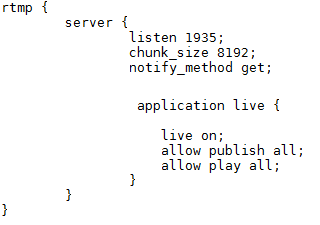
\includegraphics[width=8cm]{img/conf1.PNG}
    
    \textit{\small{Figure 3.4}}
    \end{center}


\begin{tabbing}
\hspace{4cm}\=\hspace{2cm}\=\kill
\\
\textbf{rtmp :} \> Bloc qui contiendra tous les paramètres du protocole RTMP.\\
\textbf{server : }\> Déclare une instance du serveur RTMP.\\
\textbf{listen :}\>  Ajout d’écoute du serveur sur le port “1935” pour les connexions RTMP.\\
\textbf{chunk\_size :}\>   Taille maximal d’un segment pour le flux de multiplexage.\\
\textbf{application :}\>   Création d’une application RTMP.\\
\textbf{live on :}\> Déclare l’application en fonctionnement, prêt à être utilisé.\\
\textbf{allow publish all :}\>   Autorise tous clients à diffuser sur l’application.\\
\textbf{allow play all :}\> Autorise tous clients à lire l’application.\\
    
    \end{tabbing}

    
    \\
    \\
    La configuration suivante est la configuration de base pour tester le fonctionnement du serveur, on verra par la suite que cette configuration sera amenée a changer pour mettre en place notre service de Streaming.
    \\
    \\
    
    \underline{Test Serveur NGINX 1 :}\\
    
    Pour prendre en compte la configuration précédemment, il est nécessaire de redémarrer le serveur, pour cela nous avons exécuté la commande suivante :\\


    \begin{center}
    
    \textit{ /usr/local/nginx/sbin/nginx -s reload}
    
    \end{center}


    \\
    Nous avons alors pu tester l’envoi d’un flux vers le serveur pour vérifier son fonctionnement.
    \\
    La configuration de base fonctionne bien.
    \\
    \\
    
    \underline{Installation du Serveur NGINX 2 :}\\
    
    Après avoir configurer le Proxy système et mis à jour les paquets sur la deuxième VM, nous avons suivi exactement la même procédure pour installer le serveur NGINX avec le module RTMP.
    \\
    \\
    
    \underline{Configuration du serveur sur Serveur2 :}\\
    
    Pour la configuration du deuxième serveur, nous avons commencer par faire une configuration de base comme sur le premier serveur pour vérifier son bon fonctionnement.
    \\
    \\
    
    \underline{Test Serveur NGINX 2 :}\\
    
    Redémarrage du serveur\rightarrow Diffusion~d’un~flux \rightarrow Serveur~2~OK\\
    
    \\
    
    \underline{Configuration de la redondance : }\\
    
    La configuration de la redondance sur nos serveur est une étape clé dans notre projet, en effet, comme nous l’avons précédemment présenté, nous allons répartir la charge sur deux serveurs, il faut donc que les deux serveurs diffuse du même flux à instant T pour pouvoir l'émettre aux clients.
    \\
    \\
    Comme nous avons pu le voir pendant la période de recherche et d’étude de la documentation du module nous allons utilisé la fonction “pull” du module.
    \\
    \\
    Nous avons donc édité notre fichier de configuration sur le Serveur NGINX 1 pour pull le flux qui recevra vers le Serveur NGINX 2.
    \textit{/usr/local/nginx/conf/nginx.conf} sur le Serveur NGINX 1 :
    \\
    \\
    
    
   \begin{center}
    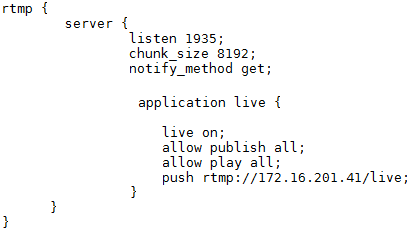
\includegraphics[width=10cm]{img/conf2.PNG}
    
    \textit{\small{Figure 4.4}}
    \end{center}    
    
    
    
    
    Pour résumer, avec cette configuration, tous les flux qui seront diffusés sur le Serveur NGINX1 sur l’application “live” seront diffusés sur le Serveur NGINX2 sur l’application live.
    \\
    \\
    
    \underline{Test de la Redondance des Serveurs :}\\

    Pour vérifier le fonctionnement de la redondance, on diffuse alors un flux vers le Serveur NGINX1, et on vérifie bien que le Serveur NGINX2 reçoit également le flux.
    \\
    \\
    A ce stade, nos deux serveurs sont donc bien configurer et prêt à être utilisé dans notre solution de Streaming.
    \\
    \\
    
    \underline{ Configuration du monitoring sur les serveurs :}
    \\
    \\
    Lors de notre phase de recherche, nous avons également vu qu’il était possible de configurer une interface de monitoring pour nos serveurs RTMP, nous avons donc configuré nos deux serveurs pour accéder à cette interface de supervision. 
    \\
    \\
    Dans nos fichiers de configuration “nginx.conf” dans la configuration du protocole HTTP nous avons rajouté :
    \\
    \\

   \begin{center}
    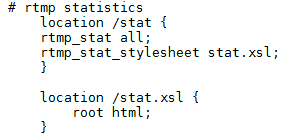
\includegraphics[width=8cm]{img/conf3.PNG}
    
    \textit{\small{Figure 5.4}}
    \end{center}

    \\
    Il ne faudra pas oublier de récupérer le template stat.xsl sur le github du module et le placer dans le répertoire html de nos serveurs (voir Webographie)
    \\
    \\
    L’interface de monitoring sera donc accessible via les adresses suivantes :
    \\
    \\
    \begin{center}
    
    \textit{Serveur NGINX1\rightarrow	http://172.16.201.40/stat}
    
    \end{center}   
    \\
    \begin{center}
    
    \textit{Serveur NGINX1\rightarrow	http://172.16.201.40/stat}
    
    \end{center}
    \\
    \\
     \begin{center}
    \textit{A ce stade, nos serveurs sont configurés et prêts à être utilisés dans notre solution de Streaming.}
    \end{center}
    \\
    \\
    \section{Mise en place d'une Régie}  
    \\
    \\
    
    Dans cette partie nous allons voir comment nous avons configuré une machine pour faire office de régie dans notre projet.
    \\
    \\
    
    \underline{Prise en main de la machine Physique en 201 :}
    \\
    \\
    
    La machine qui sera notre future régie est un PC sur Windows 7 64 bits en salle 201, celle-ci dispose d’une carte vidéo dédiée, et d’un processeur i7. Nous avons donc un accès physique à la machine.
    \\
    \\
    
    \underline{Installation d’OBS :}\\
    
    Comme nous avons pu le voir pendant la phase de recherche/test nous allons utiliser le logiciel OBS. 
    \\
    \\
    Nous avons téléchargé OBS sur le site officiel (voir Webographie)
    \\
    \\
    Et nous avons suivi une installation des plus classique.
    \\
    \\
    Lors de l’installation, OBS installe une version 32 bits et une version 64 bits, nous allons utiliser la version 64 bits.
    \\
    \\
    
    \underline{Ajout du plugin pour ouvrir les flux :}
    \\
    \\
    On télécharge le plugin sur le site communautaire  (voir Webographie) 
    \\

    \\
    Et on décompresse l’archive dans : \textit{C:\textbackslash Program Files \textbackslash OBS \textbackslash plugins}
    \\
    \\
    Une fois l'archive décompressé, on peut relancer OBS et vérifié que le plugin est bien pris en compte :
    
   \begin{center}
    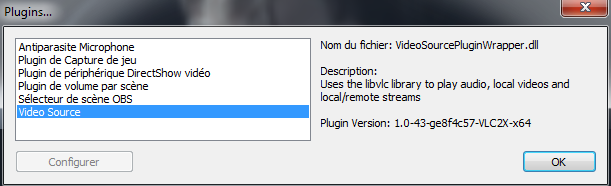
\includegraphics[width=12cm]{img/plugin2.png}
    
    \textit{\small{Figure 6.4}}
    \end{center}

    
    \underline{Ajout des sources via le plugin :}
    \\
    \\
    On peut désormais ajouter une source “video”, on va donc rajouter les flux multicast créés avec les Streamer :
    \\

    \begin{center}
    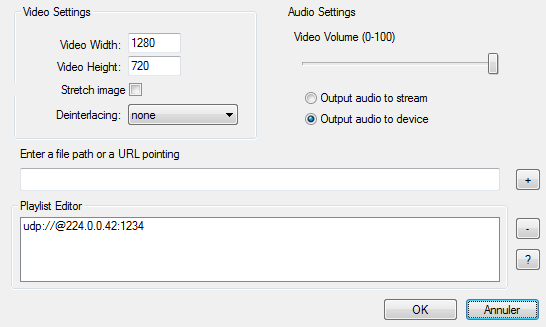
\includegraphics[width=12cm]{img/plugin.png}
    
    \textit{\small{Figure 7.4}}
    \end{center}

    \\
    Nous avons donc crée trois scènes sur OBS avec sur chaque scène une chaîne différente. OBS intègre la fonctionnalité de changer de Scène via un raccourci clavier, on peut donc (comme sur une régie) changer de chaîne via un simple raccourci clavier sans couper le direct.
    \\
    \\
    
    \underline{Configuration d’OBS :}
    \\
    \\
    Comme on a pu le voir lors de la prise en main d’OBS, il faut paramétrer OBS pour diffuser vers notre Serveur de Streaming. 
    \\
    \\
    Voilà la configuration sur notre régie :
    \\
        \begin{center}
    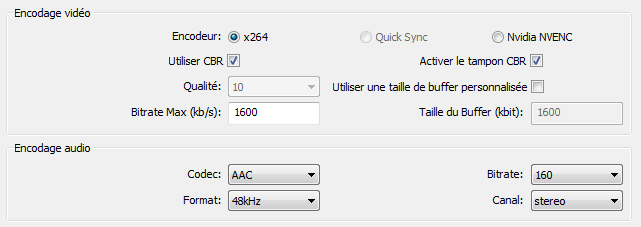
\includegraphics[width=16cm]{img/obs1.png}
    
    \textit{\small{Figure 8.4}}
    \end{center}
    
    \hfill
    
        \begin{center}
    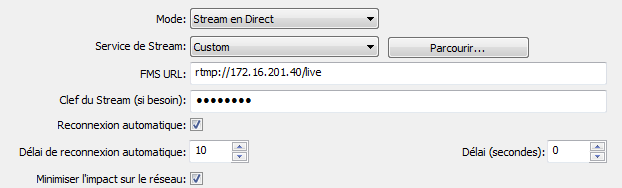
\includegraphics[width=16cm]{img/obs.png}
    
    \textit{\small{Figure 9.4}}
    \end{center}
    
    
    \\
    
    \underline{Optimisation du flux de sortie :}
    \\
    \\
    Le flux des Streamers entrant dans la régie sont des flux brutes HD qui tournent autour de 7Mb/s, il parait inconcevable de sortir un flux aussi gros vers nos serveurs et nos clients.
    \\
    \\
    Comme on peut le voir sur la figure précédente, nous utilisons la fonctionnalité "CBR" pour "Constant Bit Rate" très importante qui permet l'encodage de la vidéo avec un débit constant.
    \\
    \\
    Pour minimiser l’impact sur le réseau, et sur la machine des futurs clients, il faut donc optimiser le flux en sortie de notre régie. En effet, il faut réfléchir au meilleur ratio qualité/débit que l’on peut obtenir.
    \\
    \\
    Nous avons alors décidé lors de nos tests d’optimisation, comme on peut le voir sur les figures précédemment que nous avons configurer le flux de sortie en 720p à 60 fps avec un débit de 1600 kbits/s.
    
    \newpage
    
    \section{Développement Plate-forme Web} 
    \\
    
    \underline{Prise en main de la VM :}\\
    
    Nous avons décidé d’installer notre plateforme Web sur la dernière VM. \\

    \begin{center}

    172.168.201.42\rightarrow Serveur Web


    \end{center}
    
    \\
    \\
    
    \underline{Installation d’un Apache2 :}\\
    
    Après avoir configuré le Proxy système et mis à jour les paquets de la même manière que sur les autres VM nous avons décidé d’installer notre future plate-forme Web sur un autre serveur HTTP que NGINX, nous allons installer un Apache2 pour montrer que notre polyvalence avec les Serveurs HTTP.
    \\
    \\
    Pour se faire nous avons donc installé les paquets suivants :
    \\
    \begin{center}
    \textit{apt-get install apache2}
    \end{center}
    \\
    \begin{center}
    \textit{apt-get install apache2-utils}
    \end{center}
    \\
    \\
    \begin{center}
    La racine de notre Serveur Web sera alors : \textit{/var/www}
    \end{center}
    \\
    \hfill
    
    \underline{Développement Web de la plate-forme (Bootstrap / HTML5 CSS3) :}\\
    
     Pour développer notre plate-forme Web nous sommes partis d’un Template Bootstrap téléchargé directement sur le site officiel.
    \\
    \\
    Nous avons ensuite codé en HTML5 et CSS3 pour créer la plate-forme que nous souhaitions.
    \\
    \\
    
    \underline{Intégration d’un lecteur flash :}\\
    
    Comme nous l’avons vu lors de nos tests, il sera nécessaire d’intégrer un lecteur Flash sur notre plate-forme web pour permettre aux clients de lire notre flux Streaming.
    \\
    \\
    Nous avons alors téléchargé sur le site constructeur un player Flash (voir Webographie)
    \\
    \\
    Nous avons copié le lecteur dans un dossier “jwplayer” à la racine de notre serveur Web.

    \newpage

    Nous avons ensuite intégré le lecteur sur notre “index.html” avec le code JavaScript suivant dans le “head” :
    \\
    
    
    \begin{center}
    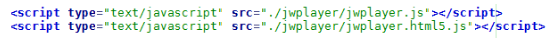
\includegraphics[width=16cm]{img/jw1.PNG}
    
    \textit{\small{Figure 10.4}}
    \end{center}
    
    
    \hfill
    
    et dans le “body” :
    \\
    
    \begin{center}
    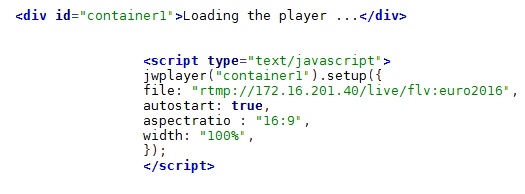
\includegraphics[width=16cm]{img/jw2.PNG}
    
    \textit{\small{Figure 11.4}}
    \end{center}
    
    \\
    On voit ici le code pour intégrer le lecteur et lire le flux du Serveur NGINX1
    \\
    \\
    \section{Mise en place du LoadBalancing}  
    
    \underline{Prise en main de la VM :}\\
    
    Nous avons décidé d’installer notre LoadBalancer sur la même VM que notre plate-forme Web, car le serveur Web et le LoadBalancer nécessite pas beaucoup de ressource. On peut donc faire tourner ces deux serveurs sur la même VM
    \\
    \\
    
        \begin{center}

    172.168.201.42 	\rightarrow 	LoadBalancer
    
        \end{center}

    \\
    \\
    \newpage
    
    \underline{Installation  d’HAPROXY :}\\
    
    Pour installer HAProxy nous avons du ajouter des sources spécifiques via la commande suivante :




    \begin{center}
    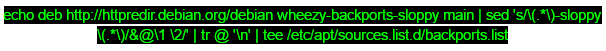
\includegraphics[width=13cm]{img/bash.PNG}
    \end{center}
    \\
    Installation du serveur HAProxy :


    \begin{center}
    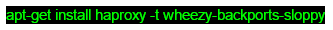
\includegraphics[width=8cm]{img/bash2.PNG}
    \end{center}
    \\
    
    \underline{Configuration d’HAPROXY :}\\
    
    Le fichier de configuration principal d’HAProxy est :\\
    
    \begin{center}
    \textit{/etc/haproxy/haproxy.cfg}
    \end{center}
    \\
    \\
    \\
    L’objectif dans la configuration de notre LoadBalancer est de rediriger les requêtes des clients vers nos deux serveurs NGINX de manière équitable.
    \\
    \\
    Pour rappel, les requêtes vers les serveurs vont être des requêtes RTMP (qui fonctionnent sur TCP)  sur le port 1935.
    \\
    \\
    Le serveur HAProxy va donc devoir écouter les requêtes TCP sur le port 1935 et les rediriger vers les deux serveurs.
    \\
    \\
    Nous avons donc édité le fichier de configuration de cette manière :
    \\

    \begin{center}
    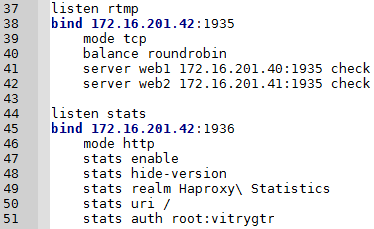
\includegraphics[width=10cm]{img/haproxy.PNG}
    
    \textit{\small{Figure 12.4}}
    \end{center}


    \\
    On voit alors sur ce fichier de configuration le protocole utilisé qui est : TCP
    \\
    \newpage
    
    On peut y voir aussi l’option “check” qui nous permet au serveur de vérifier si le serveur est UP avant d'effectuer la redirection. Si le serveur est DOWN, la redirection vers ce serveur sera annulée.
    \\
    \\
    Et pour finir on peut voir que l'on a déclaré dans le fichier de configuration une partie statistique sur le port 1936 qui va nous permettre de monitorer notre Serveur de LoadBalancing via une interface Web.
    \\
    \\
    
    \underline{Choix de l’algo de load balancing :}\\
    
    Comme on peut le voir dans le fichier de configuration ci-dessous, l'algorithme de LoadBalancing mis en oeuvre ici est “Round-Robin” c’est à dire qu’une requête sur deux sera envoyée sur l’un, puis sur l’autre (si le serveur est UP).
    \\
    \\
    
    \underline{Test du LoadBalancing :}\\
    
    Pour finir et mettre en production le LoadBalancing, nous avons désormais besoin de modifier le lien sur le lecteur qui va envoyer la requête pour le flux.
    \\
    \\
    \begin{center}
    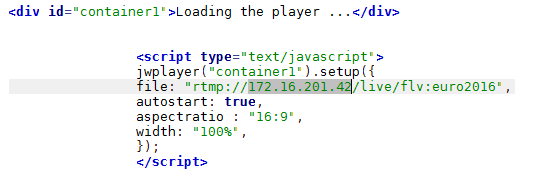
\includegraphics[width=16cm]{img/jw3.PNG}
    \textit{\small{Figure 13.4}}
    \end{center}
    

    \\
    \\
    Pour vérifier le bon fonctionnement du LoadBalancing, nous avons juste à ouvrir l’interface de monitoring sur les deux serveurs, et simuler plusieurs clients, on voit bien que le flux est envoyé une fois par le serveur NGINX1 et une fois par le serveur NGINX2.

    \newpage

    \section{Les différents clients}
    \\
    \\
    
    \underline{Client Web}\\
    
    Directement sur notre plate-forme Web via ce lien : ou http://172.16.201.42/
    \\
    \\
    Cependant, on notera qu’il est nécessaire que Flash soit installé sur le navigateur utilisé.
    \\
    \\
    
    \underline{VLC}\\
    
    Avec un lecteur qui gère les flux réseaux on peut ouvrir notre flux avec la syntaxe suivante :\\

    \begin{center}
    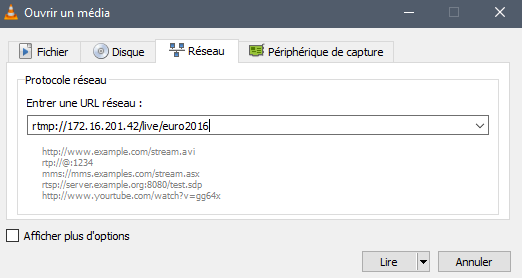
\includegraphics[width=10cm]{img/vlc.png}
    
    \textit{\small{Figure 14.4}}
    \end{center}
    
    \\


    
    \underline{	Client Xibo}\\
    
    Les écrans du hall de l’IUT ont des clients Xibo qui affichent la mise en page créée précedement pour diffuser le LiveStream.
    \\
    \\
    Nous planifions l’affichage de notre Layout chaque jour de la semaine dès le début de l’Euro de 8h à 20h.


    \begin{center}
    \textit{    “On constatera cependant que via le client Xibo il y a une baisse de framerate”}
    \end{center}
    \\
    \newpage
    
    \section{Bonus}\\
    
    Pour donner un peu plus de valeur et de logique à notre projet, nous avons demandé l’aide de Mr. SOUPRAMANIEN, le technicien de l’IUT pour mettre en place des configurations sur des système où nous n’avons pas la main.
    \\
    \\
    \underline{Entrée sur le DNS de l’IUT pour notre serveur Web}\\
    
    Mr. SOUPRAMANIEN suite à notre demande a enregistré une nouvelle entrée sur le DNS de l’IUT pour notre serveur Web.
    \\
    \\
    Entrée DNS :    eurolive	A	172.16.201.42
    \\
    \\
    Une fois la configuration appliquée sur le DNS, on peut alors accéder à notre plate-forme via l’adresse suivante :
    \\
    \\
    \begin{center}
    \underline{http://eurolive/} équivalent à \underline{http://eurolive.iutcv.fr/}
    \end{center}
    \\

    \hfill
    
    \underline{Exception sur le Proxy de l’IUT}\\
    
    Nous avons également demandé à Mr. SOUPRAMANIEN de créer une exception sur le Proxy de l’IUT pour que les futurs utilisateurs, malgré le fait qu’il ait le paramètre Proxy de l’IUT sur leur navigateur, puisse tout de même accéder à notre serveur Web.
    \\
    \\
    
    \underline{Intégration Xibo}\\
    
    Les écrans du Hall de l’IUT embarque des clients légers sous Windows. 
    \\
    \\
    L’affichage dynamique actuel est géré par Xibo, le technicien nous a alors crée un compte “étudiant” pour que l’on puisse créer notre mise en page, et planifier la diffusion de notre Live.

    
\chapter{Conclusion}

Pour conclure, nous pensons avoir eut l'opportunité de réaliser un beau et original projet durant cette année universitaire en alternance. 
\\
\\
En effet, ce projet fait l'oeuvre d'une mise en oeuvre de connaissances acquises au cours de cette formation. On y retrouve également des problématiques qui sont soulevées au quotidien dans l'écosystème d'Internet et son contenu multimédia.
\\
\\
Le fruit d'un travail collaboratif au sein de notre groupe mais aussi avec le corps enseignant, et le technicien de l'IUT pour au final, avoir un résultat des plus satisfaisant.
\\
\\
Nous sommes partie d'aucune architecture déjà mise en place à l'IUT, sur un projet où il n'y avait pas "solution" clé en main pré-existante sur Internet ou autres.
\\
\\
L'achèvement de ce projet nous permet alors d'appuyer certaines compétences techniques en parfaites harmonisation avec la formation choisie et notre futur coeur de métier.
\\
\\
Nous espérons que cela inspirera de futurs élèves universitaire dans tous leurs projets, ou dans la possible amélioration de la solution que nous avons déployée à ce jour.
\\
\\


\chapter{Glossaire}



\begin{tabbing}
\hspace{3cm}\=\hspace{2cm}\=\kill


\textbf{OBS : }  \> \textit{ Open Broadcaster Software est un logiciel Open Source et gratuit}\\ 

\textbf{VLC : } \>\textit{ VLC media player est le lecteur multimédia  Open Source}\\ 

\textbf{HTTP : }\> \textit{ HyperText Transfer Protocol}\\ 

\textbf{RTSP : } \>\textit{ Real Time Streaming Protocol}\\

\textbf{RTP : } \>\textit{ Real Time Transport Protocol}\\

\textbf{RTMP : } \>\textit{ Real Time Messaging Protocol}\\

\textbf{UDP : } \>\textit{ User Datagram Protocol}\\

\textbf{TCP :}\> \textit{ Transmission Control Protocol}\\

\textbf{MPEG : } \>\textit{ Moving Picture Experts Group}\\

\textbf{FLV : }\> \textit{ Flash Video}\\

\textbf{AAC : } \>\textit{ Advanced Audio Coding}\\

\textbf{QOS : }\> \textit{ Quality Of Service}\\

\textbf{VM : } \>\textit{ Machine Virtuelle}\\

\textbf{DNS :}\>\textit{  Domain Name System}\\

\textbf{CBR :}\>\textit{  Constant Bit Rate}\\

\textbf{NGINX : }\> \textit{ Logiciel  Open Source de Serveur HTTP }\\

\textbf{IKUSI : } \>\textit{ Entreprise Espagnol dans le domaine du multimédia}\\

\textbf{Bootstrap :}\> \textit{ Bootstrap est une librarie utile pour le développement Web}\\

\textbf{Apache2 :}\> \textit{ Logiciel  Open Source de Serveur HTTP  }\\

\textbf{HAProxy :} \>\textit{  Logiciel Open Source de Load Balancing et de Proxy serveur}\\

\textbf{GitHub : } \>\textit{ Service web d'hébergement et de gestion de développement de logiciels}\\

\textbf{Xibo :}\> \textit{ Xibo est une solution d'affichage dynamique  Open Source}\\

\textbf{Flash :} \>\textit{  Logiciel de création de contenu Multimédia}\\


\chapter{Documentations}
    \\
    \\
    
    \underline{\LARGE{Bibliographie}}
    \\
    \\
    
    \underline{Documents universitaire :}
    \\
    
    José DIAZ - Université Paris Est Créteil
    ECE33\_-\_TP1\_-\_flux\_multimedia.pdf\\


    \\
    \\

    
    \underline{\LARGE{Webographie}}
    \\
    \\
    
    \underline{Site officiel de NGINX :}\\
    \textit{https://nginx.org/}\\
    
    \\
    
    \underline{Dépôt officiel du module RTMP pour NGINX :}\\
    \textit{https://github.com/arut/nginx-rtmp-module}\\
    
    \\

    \underline{Wiki officiel du module RTMP pour NGINX :}\\
    \textit{https://github.com/arut/nginx-rtmp-module/wiki/Directives}\\
    
    \\
    

    \underline{Template officiel de Statistique pour le module RTMP :}\\
    \textit{https://github.com/arut/nginx-rtmp-module/blob/master/stat.xsl}\\
    
    \\
    
    \underline{Site officiel d'OBS :}\\
    \textit{https://obsproject.com/}\\
    
    \\

    \underline{Dépôt officiel des Plugins pour OBS :}\\
    \textit{https://obsproject.com/forum/resources/categories/plugins.3/}\\
    
    \\

    \underline{Dépôt officiel du Plugin utilisé sur OBS :}\\
    \textit{https://obsproject.com/forum/resources/video-source-plugin.20/}\\
    
    \\

    \underline{Documentation constructeur de HAProxy :}\\
    \textit{http://www.haproxy.org/download/1.3/doc/haproxy-fr.txt}\\
    
    \\

    \underline{Site avec de nombreux tutoriels sur RTMP et OBS :}\\
    \textit{https://helping-squad.com/}\\
    
    \\
      
    \underline{Site officiel du lecteur Flash utilisé :}\\
    \textit{https://www.jwplayer.com/}\\
    
    \\
    
    



     
\chapter{Annexes}


    \begin{center}
    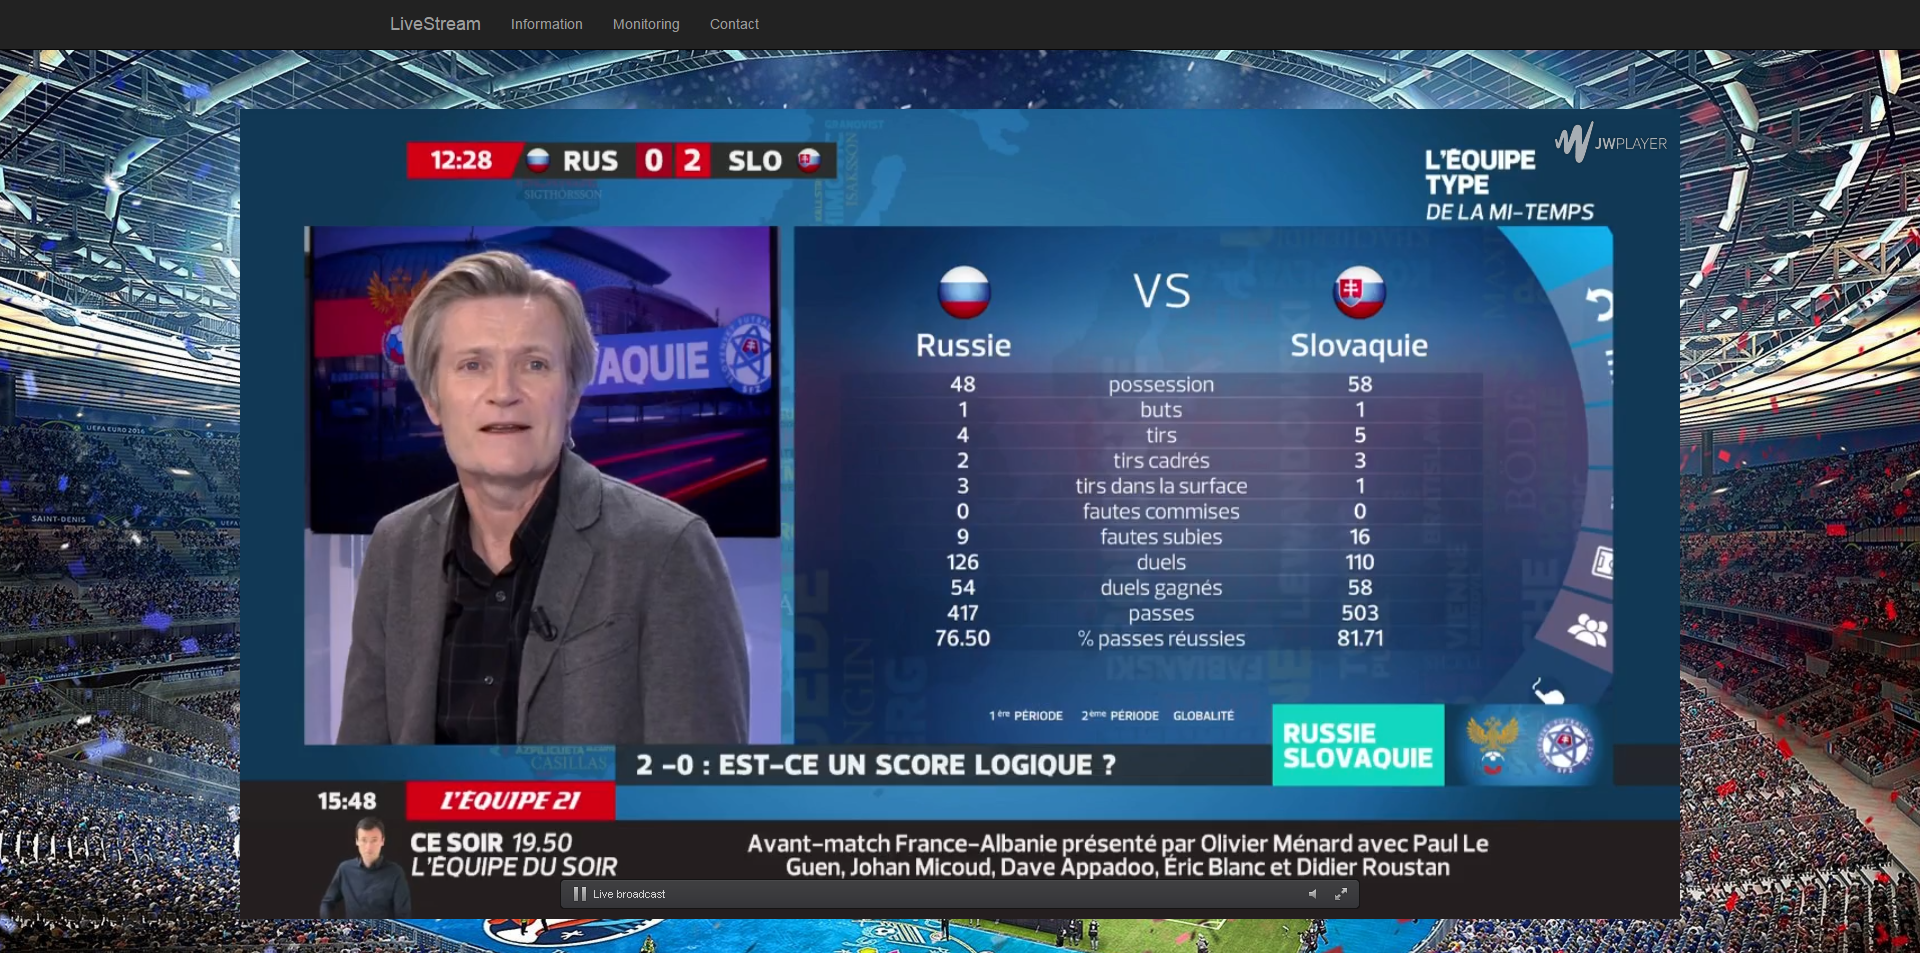
\includegraphics[width=16cm]{img/annexe2.png}
    
    \textit{\small{Accueil de notre plateforme Web avec le Live}}
    \end{center}
    
    
    
        \begin{center}
    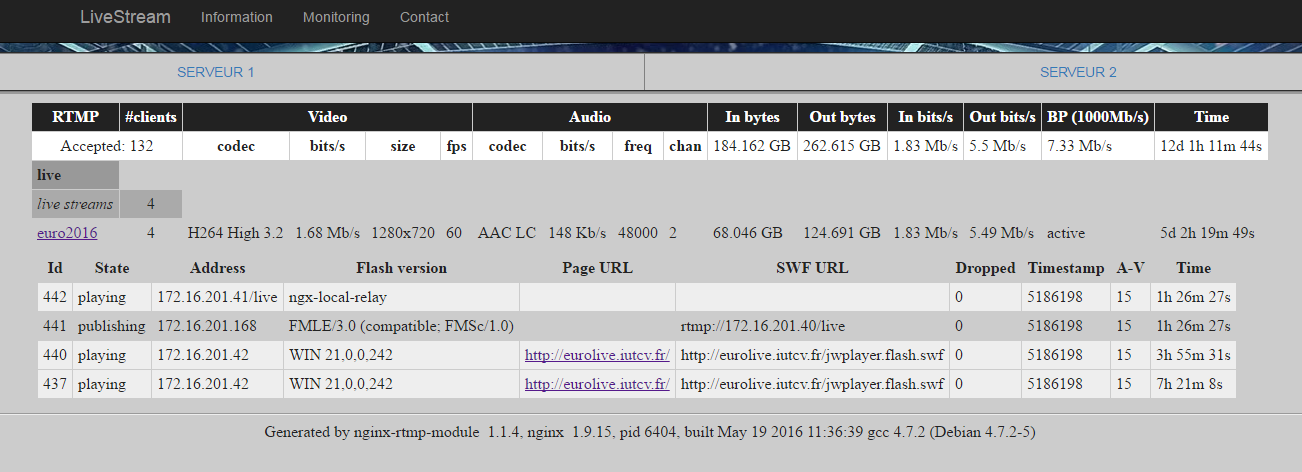
\includegraphics[width=16cm]{img/annexe1.png}
    
    \textit{\small{Interface de monitoring d'un serveur NGINX}}
    \end{center}
    


\underline{L'intégralité de notre projet est disponible sur le Github créé pour l'occasion :}

\begin{center}
\textit{https://github.com/vitry-projet-streaming/Projet\_tut\_streaming\_2015\_2016}
\end{center}



\end{document}